
\begin{figure}
\begin{subfigure}{.5\linewidth}
\centering

\begin{tikzpicture}
    \begin{axis}[
        xlabel=$|V_S|$,
        ylabel=relative time spent,
        ymode=log,
        legend style={at={(0.9,0.1)},anchor=south east},
        width=\textwidth,
		y tick label style={/pgf/number format/sci},
    ]
\addplot [mark=none, black] plot coordinates {
        (4,1) (14, 1)};


\addplot[
        mark=x,
        red,
    ] plot coordinates {
        (4,0.9961858191755759)
        (5,1.0059848034836174)
        (6,1.0015623854405225)
        (7,1.0041850516247017)
        (8,0.992834292174954)
        (9,0.9805831782750661)
        (10,1.0131070860496907)
        (11,0.9820629029946675)
        (12,0.9731684469245409)
        (13,0.9978012338195624)
};
%    \addlegendentry{DFS}


\addplot[
        mark=o,
        purple,
    ] plot coordinates {
        (4,0.9991254113598864)
        (5,1.0006304793357408)
        (6,0.9997389129846505)
        (7,1.0024122661594037)
        (8,0.9960200414287358)
        (9,0.9797204693043249)
        (10,1.006094756978359)
        (11,1.0291250941127874)
        (12,1.016228045334132)
};
%    \addlegendentry{GDFS O IP}


\addplot[
        mark=star,
        gray,
    ] plot coordinates {
        (4,1.0059277991423625)
        (5,0.9907814973218768)
        (6,1.0243229749286393)
        (7,1.020235901218478)
        (8,1.028660392466402)
        (9,0.9992951555916159)
        (10,0.9825124885953094)
        (11,0.9832292458336007)
        (12,1.0260311821681063)
        (13,1.1015279814561096)
        (14,1.0152331060942739)
};
%    \addlegendentry{GDFS C}


\addplot[
        mark=*,
        blue,
    ] plot coordinates {
        (4,1.1428023873341047)
        (5,0.8363144144880936)
        (6,0.3883692600044063)
        (7,0.12306323448284873)
        (8,0.11750735154321501)
        (9,0.05546079701782758)
        (10,0.027198570773209862)
        (11,0.09188685028611088)
        (12,0.029187752530780098)
        (13,0.028763961047358233)
        (14,0.13514762161751237)
};
%    \addlegendentry{K-Path}


\addplot[
        mark=+,
        green,
    ] plot coordinates {
        (4,1.003240741424298)
        (5,1.0007002255334068)
        (6,0.9998134962523451)
        (7,0.9954368842322697)
        (8,0.9901138150986978)
        (9,1.0994301778756659)
};
%    \addlegendentry{CP}


\addplot[
        mark=asterisk,
        magenta,
    ] plot coordinates {
        (4,1.012208101549136)
        (5,1.004540535143729)
        (6,1.006238667112502)
        (7,0.9987787321626621)
        (8,0.9857632446293185)
        (9,1.00045313105658)
        (10,0.9800057859162024)
        (11,1.0071924078562504)
        (12,1.05284665552656)
        (13,1.0473613609958743)
};
%    \addlegendentry{GDFS A IP}

 

    \end{axis}
    \end{tikzpicture}


\caption{serial}

\end{subfigure}%
\begin{subfigure}{.5\linewidth}
\centering

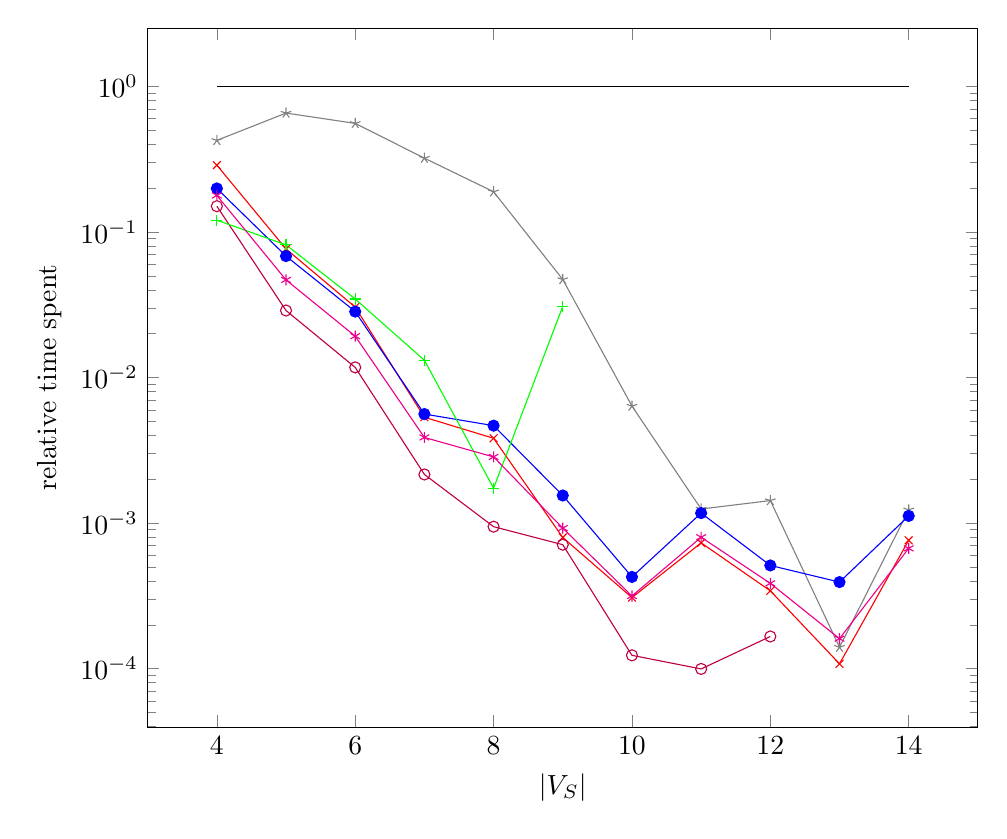
\begin{tikzpicture}
        \begin{axis}[
        xlabel=$|V_S|$,
        ylabel=relative time spent,
        ymode=log,
        legend style={at={(0.9,0.1)},anchor=south east},
        width=\textwidth,
		y tick label style={/pgf/number format/sci},
    ]
\addplot [mark=none, black] plot coordinates {
        (4,1) (14, 1)};

	

\addplot[
        mark=x,
        red,
    ] plot coordinates {
        (4,0.28797946415268216)
        (5,0.07651582579324001)
        (6,0.0304666091954765)
        (7,0.005338589440600172)
        (8,0.0038271200815995776)
        (9,7.967244945263907E-4)
        (10,3.0777658183211987E-4)
        (11,7.316319897914259E-4)
        (12,3.4267518525965546E-4)
        (13,1.0795184070755415E-4)
        (14,7.623451601108666E-4)
};
%    \addlegendentry{DFS}


\addplot[
        mark=o,
        purple,
    ] plot coordinates {
        (4,0.15049515351200515)
        (5,0.028888664846084877)
        (6,0.011744849761370135)
        (7,0.0021597185405343167)
        (8,9.451813259466757E-4)
        (9,7.108005706910614E-4)
        (10,1.2347079460250932E-4)
        (11,9.95681216803268E-5)
        (12,1.6636754548371435E-4)
};
%    \addlegendentry{GDFS O IP}


\addplot[
        mark=star,
        gray,
    ] plot coordinates {
        (4,0.4261569662504955)
        (5,0.6566221486790923)
        (6,0.5577822930842058)
        (7,0.3218592258892897)
        (8,0.18912427965228307)
        (9,0.047186436624101824)
        (10,0.006370129606168451)
        (11,0.0012501421281951863)
        (12,0.001428282896214883)
        (13,1.4047897093971695E-4)
        (14,0.0012339028104273453)
};
%    \addlegendentry{GDFS C}


\addplot[
        mark=*,
        blue,
    ] plot coordinates {
        (4,0.19921889891317368)
        (5,0.06836073093997885)
        (6,0.02840796237713794)
        (7,0.005614455272937469)
        (8,0.004672519202561842)
        (9,0.001547859891521619)
        (10,4.269626026969231E-4)
        (11,0.0011715845435014138)
        (12,5.118613622622226E-4)
        (13,3.9341491023758834E-4)
        (14,0.0011207533086203814)
};
%    \addlegendentry{K-Path}


\addplot[
        mark=+,
        green,
    ] plot coordinates {
        (4,0.12065618974765957)
        (5,0.08159990593923339)
        (6,0.03466025100832615)
        (7,0.013147623578769863)
        (8,0.0017371671223744833)
        (9,0.03084198984204367)
};
%    \addlegendentry{CP}


\addplot[
        mark=asterisk,
        magenta,
    ] plot coordinates {
        (4,0.1784159199448806)
        (5,0.04687838004113365)
        (6,0.019250300262524056)
        (7,0.003877520221788777)
        (8,0.0028497378324052747)
        (9,9.238160016552532E-4)
        (10,3.1576391186238784E-4)
        (11,7.994265736620543E-4)
        (12,3.8594286429616265E-4)
        (13,1.6073739183641855E-4)
        (14,6.707501289580087E-4)
};
%    \addlegendentry{GDFS A IP}

	
    \end{axis}
    \end{tikzpicture}

\caption{cached}

\end{subfigure}\\[1ex]
\begin{subfigure}{0.5\linewidth}
\centering

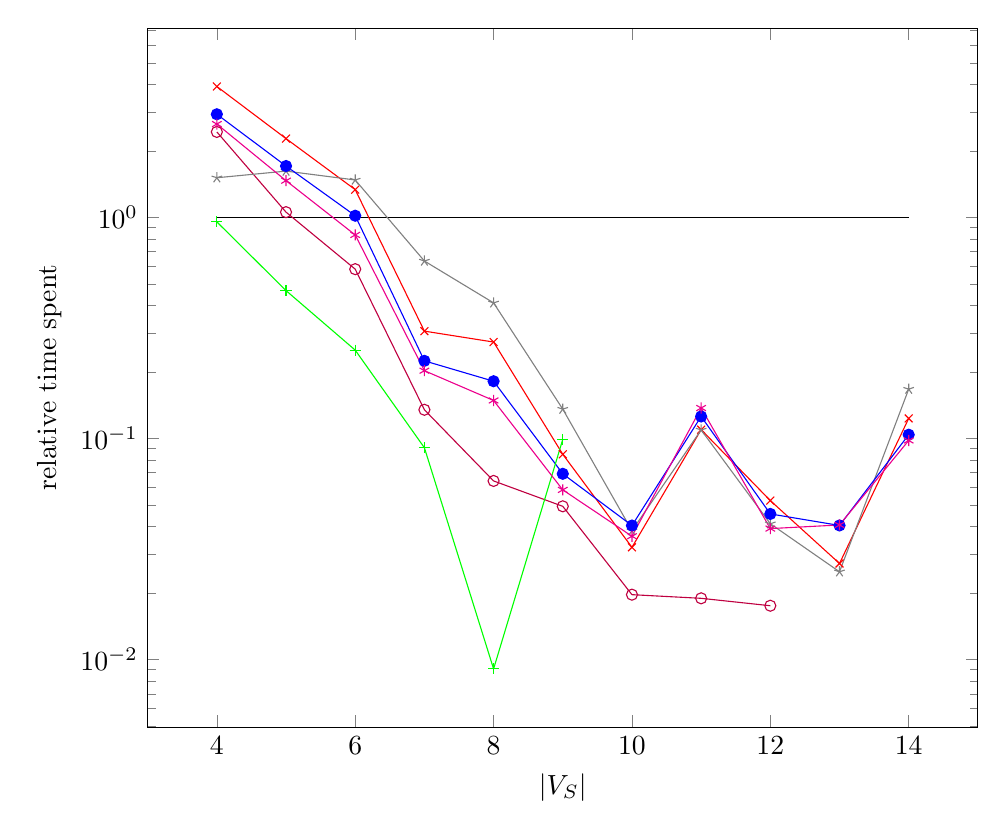
\begin{tikzpicture}
    \begin{axis}[
        xlabel=$|V_S|$,
        ylabel=relative time spent,
        ymode=log,
        legend style={at={(0.9,0.1)},anchor=south east},
        width=\textwidth,
		y tick label style={/pgf/number format/sci},
    ]
\addplot [mark=none, black] plot coordinates {
        (4,1) (14, 1)};


\addplot[
        mark=x,
        red,
    ] plot coordinates {
        (4,3.9129439575545435)
        (5,2.273222753540935)
        (6,1.3358829167973778)
        (7,0.3060292392269831)
        (8,0.27310812493561054)
        (9,0.08483478635788988)
        (10,0.03220002459721227)
        (11,0.10965821877648596)
        (12,0.05238033266084752)
        (13,0.02720606162053374)
        (14,0.12326343330507006)
};
%    \addlegendentry{DFS}


\addplot[
        mark=o,
        purple,
    ] plot coordinates {
        (4,2.4370501012142824)
        (5,1.0568408408459573)
        (6,0.5835598718338068)
        (7,0.13489675395340783)
        (8,0.06428756573066419)
        (9,0.04934951432140211)
        (10,0.01966479503287344)
        (11,0.018929462405664066)
        (12,0.01752267312020006)
};
%    \addlegendentry{GDFS O IP}


\addplot[
        mark=star,
        gray,
    ] plot coordinates {
        (4,1.5119445424232758)
        (5,1.6205884547090093)
        (6,1.4772813435520415)
        (7,0.6353071431015811)
        (8,0.41070975405654797)
        (9,0.13580170759422583)
        (10,0.03828888536206054)
        (11,0.10934140002182946)
        (12,0.0411628308005999)
        (13,0.024956633661657346)
        (14,0.16725255988991872)
};
%    \addlegendentry{GDFS C}


\addplot[
        mark=*,
        blue,
    ] plot coordinates {
        (4,2.9292287176662284)
        (5,1.7085776030673339)
        (6,1.018144876988824)
        (7,0.22453968974110117)
        (8,0.18160614741581238)
        (9,0.06924099256113281)
        (10,0.04038867770933918)
        (11,0.12581531378172073)
        (12,0.04559446907724363)
        (13,0.04043070416472683)
        (14,0.10402774643082491)
};
%    \addlegendentry{K-Path}


\addplot[
        mark=+,
        green,
    ] plot coordinates {
        (4,0.9551312671725737)
        (5,0.46672792929157314)
        (6,0.25108420813909216)
        (7,0.09084564408241347)
        (8,0.009073128728892876)
        (9,0.09911792703918121)
};
%    \addlegendentry{CP}


\addplot[
        mark=asterisk,
        magenta,
    ] plot coordinates {
        (4,2.6450452172441703)
        (5,1.466590988138647)
        (6,0.8335425887125216)
        (7,0.20265590602141004)
        (8,0.14860699155681456)
        (9,0.058559839513090184)
        (10,0.03613722819737897)
        (11,0.1373961637320401)
        (12,0.039138601300597764)
        (13,0.04064207588686031)
        (14,0.09797085693851426)
};
%    \addlegendentry{GDFS A IP}

	
    \end{axis}
    \end{tikzpicture}

\caption{parallel}

\end{subfigure}
\begin{subfigure} {0.5\linewidth}
\centering

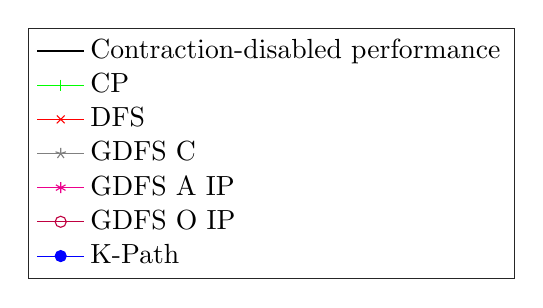
\begin{tikzpicture} 
    \begin{axis}[%
    hide axis,
    xmin=10,
    xmax=50,
    ymin=0,
    ymax=0.4,
    legend style={draw=white!15!black,legend cell align=left}
    ]
	\addlegendimage{black}
    \addlegendentry{Contraction-disabled performance}; 
     
    \addlegendimage{green, mark=+}
    \addlegendentry{CP};
    
    \addlegendimage{red, mark=x}
    \addlegendentry{DFS};
    
    \addlegendimage{gray, mark=star}
    \addlegendentry{GDFS C};
    
    \addlegendimage{magenta, mark=asterisk}
    \addlegendentry{GDFS A IP};
    
    \addlegendimage{purple, mark=o}
    \addlegendentry{GDFS O IP};
    
    \addlegendimage{blue, mark=*}
    \addlegendentry{K-Path};
    
    \end{axis}
\end{tikzpicture}

\end{subfigure}

\caption{Performance of our algorithm with \textbf{AllDifferent} pruning using \textbf{`M-filtering'} filtering relative to the performance of the algorithm without pruning. We avoid unnecessarily long paths, do not perform contraction and use the degree-based target graph vertex ordering. Data points above the black reference line denote that the pruning method introduces more delay, and data points below the reference line denote that the pruning method saves time. Note the logarithmic y-axis.}		
\label{fig:alldifferentMfiltering}
\end{figure}
